\chapter{Zásuvný modul pro QGIS}
\label{6-plugin}

\section{Tvorba QGIS zásuvného modulu}
\label{plugin-tvorba}

Do projektu Quantum GIS je možné psát zásuvné moduly v~jazycích C++ nebo Python.
Dnes už jsou častější zásuvné moduly psané v~Pythonu, přesto se však objevují
i~ty v~C++, a~to z následujících důvodů. QGIS jako takový je napsán v~tomto 
jazyce. Jedná se o~objektově orientovaný jazyk, hodí se proto pro větší projekty. 
Nevýhodou C++ pluginů je nutnost kompilace, kterou však vyváží výsledná větší 
rychlost běhu aplikace.V~případě zásuvného modulu \textit{Conflate} byl jazyk 
C++ zvolen i~z~důvodu použití knihovny \textit{GEOS}, která je psána rovněž 
v~tomto jazyce.

% zmínka o licenci? Vzhledem k tomu, že C++ pluginy většinou využívají knihovny
% libqgis*.so, které jsou publikovány pod licencí GNU GPL, musí být tyto
% moduly pod stejnou licencí.

C++ zásuvné moduly QGISu jsou dynamické knihovny (.so nebo .dll
\footnote{ přípona .so se používá v~Linuxu, přípona .dll pod systémem Windows}).
Načtení modulu v~QGISu probíhá za~běhu programu. Při startu programu 
\textit{Správce zásuvných modulů (Plugin Manager)} vyhledá všechny soubory 
s~danou příponou ve~složce se~zásuvnými moduly (v Linuxu nejčastěji /lib/qgis
nebo /usr/lib/qgis/plugins), popřípadě v~dalších složkách, jejichž umístění
je definováno v~uživatelském nastavení, a~načte je.

Pro správné načtení musí zásuvný modul obsahovat následující.

\begin{enumerate}
 \item Funkce \texttt{classFactory}, která vytvoří instanci daného pluginu.
 \item Metoda \texttt{initGui}, jejímž prostřednictvím jsou zobrazeny prvky 
	uživatelského rozhraní (ikona apod.) v~nabídce \textit{Zásuvné moduly 
	(Plugins)} a~v~liště nástrojů.
 \item Metoda \texttt{unload}, která odstraní alokované elementy a~samotnou
	instanci třídy zásuvného modulu (pomocí destruktoru) při ukončení 
	programu.
 \item Další externí C ~funkce (\texttt{name, description, ...}) pro správné
	zobrazení ve~\textit{Správci zásuvný modulů}.
\end{enumerate}

V~modulu \textit{Conflate} jsou všechny tyto funkce obsaženy ve~třídě
\texttt{QgsConflatePlugin}. 
Podrobnější popis tvorby C++ pluginu lze najít v~\textit{QGIS Coding and 
Compilation Guide} % uvést odkaz na literaturu
, odkud byly čerpány výše uvedené informace.


% pro testování konzolová aplikace
% základní informace + zásady


\section{Zásuvný modul \textit{Conflate}}
\label{plugin-navrh}
% návrh gui, funkčnost

Zásuvný modul \textit{Conflate} pro QGIS, který je jedním z~výstupů této práce,
umožňuje spojení vektorových datasetů. Pro tento proces úpravy vrstev využívá
tříd a metod výše popsané knihovny \textit{GEOC}.

Modul se skládá celkem ze~tří tříd \texttt{QgsConflateProvider}, 
\texttt{QgsConflatePlugin} a~ \texttt{QgsDialog}. Třída \texttt{QgsConflatePlugin} 
obsahuje funkce pro vytvoření a~načtení zásuvného modulu do~QGISu tak, jak bylo 
uvedeno v~kapitole \ref{plugin-tvorba}. Zobrazování a~interakci s~uživatelem 
zajišťuje třída \texttt{QgsDialog}. Konečně třída \texttt{QgsConflateProvider} 
se stará o~funkcionalitu aplikace a~obsahuje tak funkce využívající knihovnu 
\textit{GEOC} i~další funkce pro kopírování vrstvy, změnu geometrie, výpis 
protokolu apod.

\vspace{0.5cm}
\label{schema}
  \begin{figure}[hbt]
    \centering
      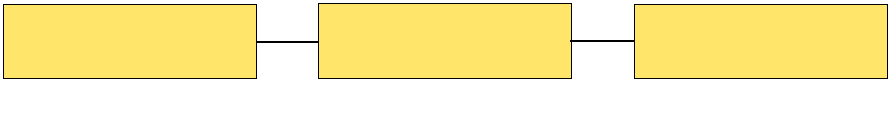
\includegraphics[width=350pt]{./pictures/schema.pdf}
      \caption{Architektura zásuvného modulu \textit{Conflate}}
      \label{fig:schema}
  \end{figure} 

%Grafické rozhraní je navrženo tak, aby splňovalo zásady tvorby uživatelského
%rozhraní dle ... % odkaz na literaturu. ...
%Vzhled dialogu byl vytvořen pomocí nástroje QT Designer.

Následuje výčet činností probíhajících při spuštění a~použití \textit{Conflate}.
Tento výčet má za~úkol pouze zprostředkovat čtenáři představu, jak modul funguje.
Podrobný návod pro jeho použití z~hlediska uživatele je pak rozepsán v~příloze
v~uživatelské příručce. Popis jednotlivých metod zas lze nalézt v~anglické
dokumentaci k~pluginu. % doplnit odkazy na přílohy

\begin{enumerate}
 \item Při otevření dialogu se do~rozbalovací nabídky načtou názvy vrstev 
	otevřených v~programu.
 \item Dalším krokem je výběr vrstev a~nastavení možností uživatelem.
 \item Po~spuštění zpracování se nejdříve zkopíruje upravovaná vrstva 
	(\textit{Subject layer}) do~nové vektorové vrstvy pomocí funkce 
	\texttt{copyLayer}. Formát nové vrstvy je vždy \textit{shapefile}
	\footnote{ESRI Shapefile je datový formát pro ukládání vektorových 
	  prostorových dat  vyvinutý firmou Esri, jedná se o~jeden 
	  z~nejrozšířenějších formátů dat pro geografické informační systémy,
	  přípona souborů v tomto formátu je .shp}.
	Tato vrstva je vytvořena v~aktuální složce a~její název odpovídá vzoru 
	\begin{center}
	 \texttt{nazev\_puvodni\_vrstvy(nejnizsi\_nepouzite\_cislo).shp},
	\end{center}
	např. \texttt{subject(3).shp}.
 \item Poté je převedena geometrie prvků zvolených vrstev (upravovaná
	a~referenční) na~reprezentaci geometrie knihovny \textit{GEOC},
	tedy z~\texttt{QgsGeometry} na~\texttt{GEOCGeometry}. Tyto geometrie
	jsou uloženy do~vektorů, které se pak předají třídám \textit{GEOC}.
 \item Jak už bylo naznačeno, je vytvořena instance příslušné třídy 
	\textit{GEOC} a~té jsou předány parametry - vektory s~prvky vybraných
	vrstev a~toleranční vzdálenost. 
 \item Dále je zavolána funkce vytvořené třídy pro zarovnání datasetů. Při volbě 
	přichycení vrcholů \textit{Snap vertices} v~dialogu je použita třída 
	\texttt{VertexSnapper} a~metoda \texttt{snap}, při volbě zarovnání 
	vrstev \textit{Coverage Alignment} pak 	třída \texttt{CoverageAlignment} 
	a~metoda \texttt{align}. Výsledek je uložen do~nového vektoru geometrií.
 \item Na závěr je upravena geometrie nové vrstvy (kopie upravované vrstvy) dle
	výsledků úprav provedených algoritmy knihovny \textit{GEOC}.
 \item Nová vrstva se automaticky přidá do~aktuálního projektu v~QGISu a~zobrazí
	se v~panelu \textit{Vrstvy (Layers)}.
 \item Po~zpracování vrstvy se do textového okna dialogu vypíše protokol 
	o~zpracování, který obsahuje název vstupních a~výstupních dat, počet
	zpracovácaných prvků a~počet nevalidních prvků včetně výpisu jejich
	identifikátorů (\textit{id}).
\end{enumerate}


\section{Ukázky}
\label{plugin-ukazky}
% obrázky s popisem funkcionality


\section{Uživatelská příručka} %% přesunout do příloh
\label{prirucka}

Tato příručka je psána pro použití modulu \textit{Conflate} s~Quantum GIS 1.9.0 , 
v~jiných verzích se může způsob načtení modulu, popř. i~jiné činnosti mírně lišit.

\subsection{Instalace}
\label{prirucka-instalace}
Instalace ... Je potřeba knihovna \textit{GEOC} ..


\subsection{Načtení zásuvného modulu}
\label{prirucka-nacteni}

Načtení zásuvného modulu lze provést ve~Správci zásuvných modulů.
\begin{center}
\textit{Zásuvné moduly~$\rightarrow$~Spravovat~zásuvné~moduly... 
(Plugins~$\rightarrow$~Plugin Manager...)}
\end{center}
Zde je třeba zaškrtnout \textit{Conflate Plugin}. Po~provedení tohoto kroku by se 
měla objevit ikonka modulu v~nástrojové liště a~také v~menu \textit{Zásuvné moduly}. 
Pokud se plugin nezobrazuje ve~Správci zásuvných modulů, je třeba nastavit cestu 
k~souboru~.so v~\textit{Nastavení}.
\begin{center} 
\textit{Nastavení~$\rightarrow$~Volby~$\rightarrow$~Systém~$\rightarrow$~Cesty 
k~zásuvným modulům (Settings~$\rightarrow$~Options$\rightarrow$~System~$\rightarrow$
~Plugin paths)}
\end{center}


\subsection{Spuštění a nastavení dialogu}
\label{prirucka-spusteni}

Před spuštěním dialogu \textit{Conflate} je třeba mít v~aktuálním projektu 
načteny vrstvy, které chceme zpracovávat. Po~otevření dialogu je třeba provést 
výběr \textbf{referenční vrstvy} (\textit{Reference Layer}) a~\textbf{upravované 
vrstvy} (\textit{Subject Layer}). Referenční vrstva je obvykla ta s~vyšší 
přesností, která se nebude měnit. Upravovanou vrstvu naopak chceme zarovnat 
k~vrstvě referenční.

Dále je třeba nastavit \textbf{toleranční vzdálenost} (\textit{Distance 
Tolerance}) v~jednotkách projektu. Tato vzdálenost udává, v~jaké maximální 
vzdálenosti mohou být odpovídající si prvky z~obou vrstev a~zároveň, jak 
moc se tedy může cílová vrstva měnit. V~ideálním případě by tato vzdálenost 
neměla přesahovat nejkratší segment geometrie všech prvků upravované vrstvy 
(tzn. nejkratší úsek linie, nejkratší stranu polygonu). Nevhodná volba této 
vzdálenosti může vést ke~vzniku nevalidních geometrií či nereálným výsledkům.

Nakonec je nutné zvolit způsob zpracování (\textit{Select the way of conflation}). 
Na~výběr jsou tyto metody:
\begin{itemize}
 \item \textbf{Přichycení vrcholů} (\textit{Snap Vertices}) - tato metoda vyhledá 
	blízké vrcholy z~obou datasetů a~změní polohu bodů upravované vrstvy tak, 
	aby odpovídala poloze blízkých bodů vrstvy referenční.
% obrázek, jak funguje ?
 \item \textbf{Zarovnání vrstev} (\textit{Coverage Alignment}) - princip této 
	metody je složitější. Na~rozdíl od~předchozí metody nepracuje s~jednotlivými
	body, ale s celými prvky. Upravuje i~některé prvky, k nimž neexistují 
	žádné odpovídající ve~vrstvě refe\-renční, a~to na~základě změny okolních 
	prvků. Je proto vhodnější zejména pro datasety, které mají rozdílný počet
	prvků. Obecně je možné s~touto metodou dosáhnout přesnějších a~často
	reálnějších výsledků, avšak na~úkor času zpraco\-vání.
% obrázek, jak funguje ?
\end{itemize}

Volba toleranční vzdálenosti a~metody zarovnání může výrazně ovlivnit rychlost 
zpracování, je proto doporučeno volit raději vždy menší vzdálenost a~jednodušší
metodu a~teprve po zobrazení výsledků případně parametry změnit. Po~nastavení 
všech parametrů se stisknutím tlačítka \textit{Process} spustí zpracování. 

\subsection{Výsledek}
\label{prirucka-vysledek}

Upravená vrstva se uloží jako nová vrstva formátu \textit{shapefile} do~aktuálního 
adresáře a~zároveň se automaticky přidá do~otevřeného projektu v~QGISu.

V~dialogu zásuvného modulu se do~textového pole vypíše protokol o~zpracování.
Formát protokolu je popsán na~obrázku \ref{fig:protokol}.  

\label{protokol}
  \begin{figure}[hbt]
    \centering
      \includegraphics{./pictures/protokol.pdf}
      \caption{Formát protokolu}
      \label{fig:protokol}
  \end{figure} 

Výsledkem zpracování mohou být i~nevalidní geometrie, jejichž identifikátory lze
nalézt v~protokolu. Proto jsou často nezbytné ještě závěrečné úpravy s~využitím
editačních nástrojů QGISu. 